\chapter{Description of CC-EKF-SLAM}\label{ch:algorithm}

The proposed algorithm: Camera Centric EKF SLAM (CC-EKF-SLAM), is
described in this chapter. Its preliminary test result on real flight
data was published in \cite{zhang_obstacle_2012}. The algorithm was
implemented in Python programming language\cite{_python_????}. An open
source machine vision library OpenCV\cite{_opencv_????} was utilized
to perform machine vision tasks such as feature extraction and
tracking. The Shi-Tomasi corner detector \cite{shi_good_1994} was used
to extract corner features from the image sequence. Feature tracking
was accomplished through the pyramid implementation of the Lucas-Kanade
optical flow method \cite{bouguet_pyramidal_1999}.

\section{Camera Centric Inverse Depth Parameterization}
Figure \ref{fig:algo1} shows the landmark parameters definition in inverse
depth parameterization.

\begin{figure}[h]
\centering
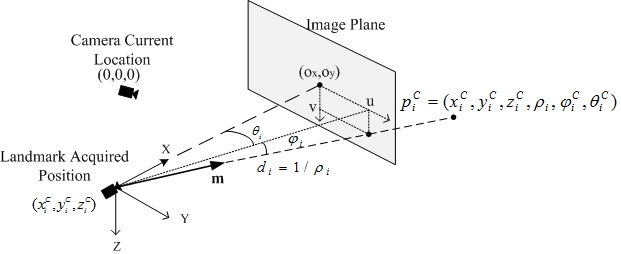
\includegraphics[width=10cm, keepaspectratio=true]{./Figures/idp.jpg}
\caption{Inverse depth parameterization}
\label{fig:algo1}
\end{figure}

\noindent A 3D scene point $\boldsymbol{p_{i}^{C}}$ can be defined by 6 parameters
with $i$ representing the landmark number. The superscript $C$
indicates that the parameters are represented in the camera reference frame.
\begin{equation}
\boldsymbol{p_{i}^{C}}=\begin{bmatrix}
x_{i}^{C} & y_{i}^{C} & z_{i}^{C} & \rho _{i} & \varphi _{i}^{C} & 
\theta _{i}^{C} 
\end{bmatrix}
\end{equation}
The first three parameters $[x_{i}^{C}, y_{i}^{C}, z_{i}^{C}]$
represent the initialization point where the landmark is first observed.
$\rho_{i} = 1/d_i$ is the inverse distance from the initialization position
to the landmark. The elevation-azimuth pair $[\varphi_{i}^{C},
\theta_{i}^{C}]$ encodes a unit vector pointing from the
initialization point to the landmark. The vector is given by
\begin{equation}
\label{eq:m}
\vec{\boldsymbol{m}}(\varphi_{i}^{C}, \theta_{i}^{C})=\begin{bmatrix}
\cos\varphi_{i}^{C}\cos\theta _{i}^{C} \\
\cos\varphi_{i}^{C}\sin\theta _{i}^{C} \\
\sin\varphi_{i}^{C}
\end{bmatrix}
\end{equation}

\noindent Given the a vector $[h_x, h_y, h_z]$, one can also find the
elevation-azimuth angles $[\varphi, \theta]$ by

\begin{equation}
\label{eq:m_inv_varphi}
\varphi 
=arctan\left(\frac{h_{z}}{\sqrt{h_x^2+h_y^2}}\right)
\end{equation}

\begin{equation}
\label{eq:m_inv_theta}
\theta =arctan\left(\frac{h_{y}}{h_{x}}\right)
\end{equation}


\section{Modeling the System with Extended Kalman 
Filter}

\subsection{Full State Vector}

The EKF full state vector is defined as 

\begin{equation}
\boldsymbol{x}=\begin{bmatrix}
\boldsymbol{OX_{W}^{C}} & \boldsymbol{c^{C}} & \boldsymbol{r^{C}} & 
\boldsymbol{p_{1}^{C}} & \boldsymbol{p_{2}^{C}} & \ldots 
\end{bmatrix}^T
\end{equation}

\noindent where $\boldsymbol{OX_{W}^{C}}= \begin{bmatrix}O_{x}^{C} &
  O_{y}^{C} & O_{z}^{C} & W_{x}^{C} & W_{y}^{C} &
  W_{z}^{C} \end{bmatrix}^{T}$ contains translation parameters
$\boldsymbol{O_{x,y,z}^{C}}$ and orientation parameters
$\boldsymbol{W_{x,y,z}^{C}}$ that represent the world frame position and
orientation referenced to the camera frame.
$\boldsymbol{c^{C}}$ and $\boldsymbol{r^{C}}$ represent the camera
translation and rotation motion frame by frame. $\boldsymbol{p_{i}^{C}}$
contains the $i^{th}$ landmark parameters described in the previous section.

\subsection{Prediction}

For a prediction step at time $k$, the world frame parameter
$\boldsymbol{OX_W^C}$ and landmarks parameters $\boldsymbol{p_i^C}$ are kept
unchanged from time $k-1$. The camera parameters are updated using the
new inertial measurements: velocity $\boldsymbol{v^{C}}$, acceleration
$\boldsymbol{a^{C}}$, and rate of change $\boldsymbol{w^{C}}$ in roll, pitch, and
azimuth. The full state vector at time $k$ is
\begin{equation}
\boldsymbol{\hat{x}_{k}^-}
=\begin{bmatrix}
\boldsymbol{OX_{W,k-1}^{C}} & 
\boldsymbol{c_{measured}^{C}} &
\boldsymbol{r_{measured}^{C}} & 
\boldsymbol{p_{1,k-1}^{C}} & 
\boldsymbol{p_{2,k-1}^{C}} & 
\ldots & 
\boldsymbol{p_{n,k-1}^C}
\end{bmatrix}^T
\end{equation}

\noindent where 

$$\boldsymbol{c_{measured}^{C}}=\boldsymbol{v_{measured}^{C}}\Delta t+ 
\frac{1}{2}\boldsymbol{a_{measured}^{C}}\Delta t^{2}$$
$$\boldsymbol{r_{measured}^{C}}=\boldsymbol{r_{k-1}^{C}}+ \boldsymbol{w_{measured}^{C}}$$

\noindent and $\Delta t$ is the time elapsed from frame to frame. 

\subsection{Measurement Model}

Each observed landmark is related to the camera motion through the
measurement model (Figure \ref{fig:measurement_model}). This
relationship enables a correction on the camera motion and landmark
parameters based on the landmark locations observed in the image.

\begin{figure}[h]
\centering
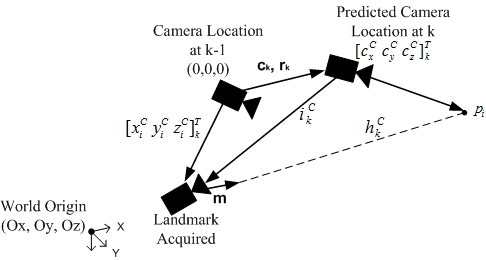
\includegraphics[width=12cm, keepaspectratio=true]{./Figures/measurement_model.jpg}
\caption{Measurement model}
\label{fig:measurement_model}
\end{figure}
\FloatBarrier
For a landmark $\boldsymbol{p_{i}^{C}}$, the vector $\boldsymbol{i^{C}}$
pointing from the predicted camera location to the landmark
initialization position is

\begin{equation}
\boldsymbol{i_{k}^{C}}=\begin{bmatrix}
x_{i}^{C} \\
y_{i}^{C} \\
z_{i}^{C} \\
\end{bmatrix}_{k}-\begin{bmatrix}
c_{x}^{C} \\
c_{y}^{C} \\
c_{z}^{C} \\
\end{bmatrix}_{k}
\end{equation}

The normalized vector pointing from the predicted camera position to the 
landmark at time k is then 
\begin{equation}
  \boldsymbol{h_{k}^{C}}=\boldsymbol{Q}^{-1}\left(\boldsymbol{r_{k}^{C}}\right)
  \left(\rho_{k}\boldsymbol{i_{k}^{C}}+
    \boldsymbol{m}\left(\varphi_k^{C},\theta _{k}^{C}\right)\right)
\end{equation}

\noindent where $\boldsymbol{Q}^{-1}(\boldsymbol{r_{k}^{C}})$ is the inverse
rotation matrix from the camera frame at time $k-1$ to camera frame at
time $k$. From vector $\boldsymbol{h_{k}^{C}}$, the landmark location on
image plane can be found by

\begin{equation}
\boldsymbol{h_{k}^{U}}= \begin{bmatrix}
u_{k} \\
v_{k} \\
\end{bmatrix}=\begin{bmatrix}
\frac{f_{x}h_{y,k}^{C}}{h_{x,k}^{C}} \\
\frac{f_{y}h_{z,k}^{C}}{h_{x,k}^{C}} \\
\end{bmatrix}
\end{equation}

\noindent where $f_{x}$ and $f_{y}$ is the scaling factor of the projection 
obtained through camera calibration.

Since the measurement model is non-linear, the equation must be
linearized to calculate the Kalman gain $K$. The detailed formulation for
linearization is given in Appendix \ref{sec:jac_measurement}.

\subsection{Composition}

The corrected state vector has all its parameters defined in camera
frame at time $k-1$. To keep the reference frame up-to-date, a coordinate
transformation is needed to transform all parameters, and the error matrix
into camera frame at step k so that the next cycle of tracking can be
continued. This step is referred to as the composition. To
differentiate the camera frame, a subscript $k$ and $k-1$ are added to
the reference frame indicator $C$.

World reference frame parameters are transformed using the equation

\begin{equation}
\begin{bmatrix}
O_{x}^{C_{k}} \\
O_{y}^{C_k} \\
O_{z}^{C_k} \\
\end{bmatrix}_{k}=\boldsymbol{Q}^{-1}(\boldsymbol{r_{k}^{C_{k-1}}})\left(
\begin{bmatrix}
O_{x}^{C_{k-1}} \\
O_{y}^{C_{k-1}} \\
O_{z}^{C_{k-1}} \\
\end{bmatrix}_{k}- \begin{bmatrix}
c_{x}^{C_{k-1}} \\
c_{y}^{C_{k-1}} \\
c_{z}^{C_{k-1}} \\
\end{bmatrix}_{k}\right)
\end{equation}

\noindent and
\begin{equation}
\begin{bmatrix}
W_{x}^{C_{k}} \\
W_{y}^{C_{k}} \\
W_{z}^{C_{k}} \\
\end{bmatrix}_{k}= \begin{bmatrix}
W_{x}^{C_{k-1}} \\
W_{y}^{C_{k-1}} \\
W_{z}^{C_{k-1}} \\
\end{bmatrix}_{k}-\boldsymbol{r_k^{C_{k-1}}}
\end{equation}
 
Landmark parameters are related to the previous reference frame by

\begin{equation}
\begin{bmatrix}
x_{i}^{C_{k}} \\
y_{i}^{C_{k}} \\
z_{i}^{C_{k}} \\
\end{bmatrix}_{k}=\boldsymbol{Q}^{-1}(\boldsymbol{r_k^{C_{k-1}}})\left(
\begin{bmatrix}
x_{i}^{C_{k-1}} \\
y_{i}^{C_{k-1}} \\
z_{i}^{C_{k-1}} \\
\end{bmatrix}_{k}- \begin{bmatrix}
c_{x}^{C_{k-1}} \\
c_{y}^{C_{k-1}} \\
c_{z}^{C_{k-1}} \\
\end{bmatrix}_{k}\right)
\end{equation}

\noindent and
\begin{equation}
\begin{bmatrix}
\rho_{i} \\
\varphi_{i}^{C_{k}} \\
\theta_{i}^{C_{k}} \\
\end{bmatrix}_{k}=
\begin{bmatrix}
\rho _{i} \\
\boldsymbol{m}^{-1}\left(\boldsymbol{Q}^{-1}(\boldsymbol{r_k^{C_{k-1}}})\boldsymbol{m}(\varphi _{i, k}^{C_{k-1}}, \theta _{i, k}^{C_{k-1}})\right) \\
\end{bmatrix}
\end{equation}

\noindent where $\rho_i$ is a scalar that doesn't require transformation.
$\boldsymbol{m}^{-1}$ represents the operator that converts
a unit vector back to $[\varphi, \theta]$ angles as defined in
Equations (\ref{eq:m_inv_varphi}) and (\ref{eq:m_inv_theta}).

The covariance matrix is also affected by this transformation. The new
covariance matrix is related to the old one by

\begin{equation}
\boldsymbol{P_{k}^{C_{k}}}=\boldsymbol{J_{C_{k-1}\to C_{k}}}\boldsymbol{P_{k}^{C_{k-1}}}\boldsymbol{J_{C_{k-1}\to C_{k}}^{T}}
\end{equation}

\noindent where $\boldsymbol{J_{C_{k-1} \to C_k}}$ is the Jacobian matrix of the
composition equations. Detail derivation of the Jacobian matrix is
given in Appendix \ref{sec:jac_composition}  

\subsection{Filter Initialization} \label{sec:filter_initialization}
\subsubsection{State Vector}

The state vector is initialized at the first frame. The world frame
position and orientation, camera motions, and the landmark
initialization points are all initialized to zero, with variance
equal to the smallest machine number.

\begin{equation}
\label{eq:OX_init}
\boldsymbol{OX_{W}^{C}}=\begin{bmatrix}0&0&0&0&0&0\end{bmatrix}^T 
\end{equation}

\begin{equation}
\boldsymbol{c^{C}}=\begin{bmatrix}0&0&0\end{bmatrix}^T
\end{equation}

\begin{equation}
\boldsymbol{r^{C}}=\begin{bmatrix}0&0&0\end{bmatrix}^T
\end{equation}

\begin{equation}
\label{eq:pi_init}
\boldsymbol{p_{i}^{C}}=\begin{bmatrix}0&0&0&\rho _{i}&\varphi_{i}^C&\theta_{i}^C\end{bmatrix}^T
\end{equation}

The inverse distance $\rho$ of all landmarks are initialized to 0.01
($d=100 meters$). The landmark elevation-azimuth angles $[\varphi _{i}^{C},
\theta _{i}^{C}]$ are extracted from landmark coordinates in the image
plane. A vector pointing from camera optical center to a landmark
can be defined by
\begin{equation}
\label{eq:init_landmark_unit_vec}
\boldsymbol{h^{C}}=\begin{bmatrix}
h_{x}^{C}\\
h_{y}^{C}\\
h_{z}^{C}\\
\end{bmatrix}
 = \begin{bmatrix}
1 \\
(u-c_x)/f_{x} \\
(v-c_y)/f_{y} \\
\end{bmatrix}
\end{equation}

\noindent where $[u, v]$ are the landmark coordinates in the image, $
[f_{x}, f_{y}]$ are the scaling factors of the projection from the scene
to the image plane, $[c_x, c_y]$ are the coordinates at which the optical axis
intersects the image plane. The elevation-azimuth angles $[\varphi
_{i}^{C}, \theta _{i}^{C}]$ can be directly calculated from
$\boldsymbol{h^{C}}$ using Equations (\ref{eq:m_inv_varphi}) and (\ref{eq:m_inv_theta})

\subsubsection{State Covariance Matrix}

As the world reference frame is defined by the camera reference frame
at time 0, it allows the filter to be initialized with minimum
variance, which helps to reduce the lower bound of the filter error
according to the EKF SLAM properties. The initial covariance matrix for the
world reference frame position and orientation, and the camera motion is

\begin{equation}
\label{eq:Pinit}
\boldsymbol{P}=\boldsymbol{I_{12\times 12}}\cdot \epsilon 
\end{equation}

\noindent where $\epsilon $ is the least significant bit (LSB) of a
computer.

The covariance of landmarks are added one by one as there is 
correlation between them. For every new landmark added, the new 
covariance matrix becomes

\begin{equation}
\label{eq:Pnew}
\boldsymbol{P_{new}}=\boldsymbol{J}\begin{bmatrix}
\boldsymbol{P_{old}} & \boldsymbol{0} \\
\boldsymbol{0} & \boldsymbol{R} \\
\end{bmatrix}
\boldsymbol{J}^{T}
\end{equation}

\noindent where $\boldsymbol{P_{old}}$ is the covariance matrix of the existing
state vector. The initial $\boldsymbol{P_{old}}$ before the addition of the first landmark is Equation (\ref{eq:Pinit}). Matrix $\boldsymbol{R}$ is given by.

\begin{equation}
\label{eq:R}
\boldsymbol{R}=\begin{bmatrix}
\sigma _{x_{i}^{C}} & & & & & & \\
 & \sigma _{y_{i}^{C}} & & & 0 & & \\
 & & \sigma _{z_{i}^{C}} & & & & \\
 & & & \sigma _{\rho } & & & \\
 & 0 & & & \sigma _{image} & & \\
 & & & & & \sigma _{image} & \\
\end{bmatrix}
 = \begin{bmatrix}
\epsilon & & & & & & \\
 & \epsilon & & & 0 & & \\
 & & \epsilon & & & & \\
 & & & 0.01 & & & \\
 & 0 & & & 1 & & \\
 & & & & & 1 & \\
\end{bmatrix} 
\end{equation}

\noindent where $[\sigma_{x_{i}}^{C}, \sigma_{y_{i}}^{C}, \sigma
_{z_{i}}^{C}]$ is the uncertainty of the camera optical center
position, initialized to $\epsilon$. $\sigma_{image}$ is the variance
of the landmark coordinate on the image plane, set to 1 pixel. $\sigma
_{\rho }$ is the uncertainty of the inverse distance. Because the
filter mainly deals with distant landmark, $ \sigma _{\rho }$ is
initialized to 0.01 to cover distances from 50 meters to infinity.

$\boldsymbol{J}$ in Equation (\ref{eq:Pnew}) is the Jacobian matrix
for the landmark initialization equations given in Equations
(\ref{eq:OX_init})-(\ref{eq:pi_init}), (\ref{eq:m_inv_varphi}), and
(\ref{eq:m_inv_theta}). Detailed formulation of the Jacobian matrix is
given in Appendix \ref{ch:appendix2}.



\subsection{Adding and Deleting Landmarks}
To shorten processing time for each iteration, landmarks that moved
out of the camera's field of view (FOV) are removed from the filter
state vector and covariance matrix. The removal is done by deleting
the parameters from the state vector, and the related rows and columns
of the state covariance matrix. All tracked landmarks are recorded
into a database. The deleted landmarks have their parameters updated
based on the camera motion without any further Kalman corrections.

While some landmarks are deleted, new landmarks are added to the
filter to maintain sufficient amount of landmarks for mapping. The
landmark addition occurs after the composition step of each
iteration, and follows the same procedure as the filter
initialization described in Section \ref{sec:filter_initialization}.
The flow chart of the entire algorithm is shown in Figure
\ref{fig:flowchart}.

\begin{figure}[h]
\centering
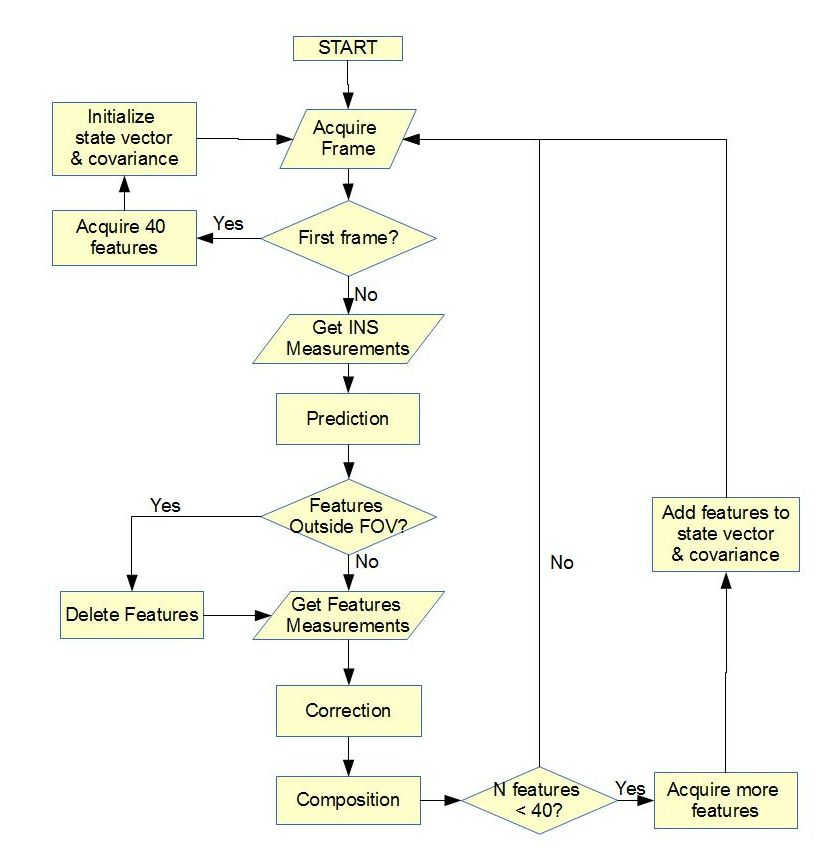
\includegraphics[width=14cm, keepaspectratio=true]{./Figures/flow_chart.jpg}
\caption{Algorithm flow chart}
\label{fig:flowchart}
\end{figure}
\FloatBarrier
% \subsubsection{Bundle Correction with GPS (not yet implemented)}
% Apply overall correction on the map at a sparser time interval using the 
% GPS positions. 

\section{Additional Procedures for Data Analysis}
% word checked.
To compare the estimated SUAS poses and landmark positions to the ground
truth, all data must be referenced to the same reference frame. For
ease of viewing, the reference frame used for data analysis is the
world frame defined by the camera frame at time 0. 

The longitude and latitude of the SUAS position were first converted
to UTM using the WGS84 world geodetic system \cite{_world_????}. Many
software packages are readily available to do the conversion by taking GPS
coordinates and zone number as input. The software used in this work is
a Python interface to PROJ.4 library \cite{_pyproj_????} called pyproj
\cite{_pyproj_????}. Secondly, the ground truth of the SUAS positions
were brought to the world frame by reference frame transformation.

$$\text{True SUAS position}^W = 
Q_{step2}^{-1}Q_{step1}^{-1} \cdot\text{SUAS position}^{UTM}$$

\noindent where $Q_{step1}^{-1}$ and $Q_{step2}^{-1}$ is the inverse
transformation matrix for a reference frame evolving from UTM to world
frame. The formulation for coordinate transformation is given in
Appendix \ref{ch:appendix1}. The UTM to world frame transformation is
illustrated in Figure \ref{fig:utm_to_world}, and the transformation
parameters for step 1 and step 2 are also listed.

\begin{figure}[h]
  \centering
  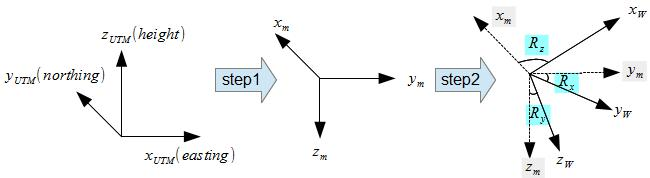
\includegraphics[width=12cm,keepaspectratio=true]{./Figures/utm_to_world.jpg}
  \caption{Coordinate transformation from UTM to world frame}
  \label{fig:utm_to_world}
\end{figure}

$$T_{step1} = \begin{bmatrix}Easting_{init}, Northing_{init},
  Height_{init}\end{bmatrix}$$
$$R_{step1} = \begin{bmatrix}180^{\circ}, 0^{\circ},
  -90^{\circ}\end{bmatrix}$$
$$T_{step2} = \begin{bmatrix}0, 0, 0\end{bmatrix}$$
$$R_{step2} = \begin{bmatrix}Roll_{init}, Pitch_{init},
  Azimuth_{init}\end{bmatrix}$$

\noindent where $Easting_{init}$, $Northing_{init}$,
$Height_{init}$, $Roll_{init}$, $Pitch_{init}$, and
$Azimuth_{init}$ are the SUAS's position and orientation in UTM at time 0. 

Ground truth SUAS orientations were captured by the UAV navigation
unit GS-111m. Both ground truth and estimated orientation were
represented in aircraft principal axes. Hence, for the ground truth
SUAS orientation to be compared to the estimated data, the only step
is to subtract the orientation at time 0.

$$\text{SUAS orientation}_{\text{Ground truth}} =
\text{Orientation}^{Nav} - \text{Orientation}^{Nav}_0$$

The estimated SUAS poses can be obtained from the world reference
frame estimates in the filter state vector:

$$ \text{Estimated SUAS poses} = 
[-O_{XYZ}^{C}, -W_{XYZ}^{C}]$$.


To examine the accuracy of estimated landmark positions, DEM data were
converted into the world frame following the same procedure as the SUAS
position. Landmarks estimated from the CC-EKF-SLAM algorithm were
converted to the world frame using the estimated SUAS localization results
as reference frame evolving parameters. Let $[X_i^W,Y_i^W,
Z_i^W]^T_k$ be the $i^{th}$ landmarks coordinates in world frame at
step $k$, then

\begin{equation}
  \left[ \begin{array}{c}
    X_{i}^{W}  \\
    Y_{i}^{W}  \\
    Z_{i}^{W}  \\
  \end{array} \right]_k=Q^{-1}(\boldsymbol{O_{XYZ, k}^{c}}, \boldsymbol{W_{XYZ,k}^{c}})\left(\left[
    \begin{array}{c}
      x_{i}^{C} \\
      y_{i}^{C} \\
      z_{i}^{C} \\
    \end{array}
  \right]_k+\frac{1}{\rho _{i,k}}\boldsymbol{m}(\varphi_{i,k}^{C},\theta_{i,k}^{C})\right)
\end{equation}

%%% Local Variables:
%%% mode: latex
%%% TeX-master: "thesis"
%%% End:
